\documentclass{article}
\usepackage{graphicx} % Required for inserting images
\usepackage{amsmath}
\graphicspath{ {./images/architetture-degli-elaboratori/} }

\title{
	Appunti di Architetture degli elaboratori \\
	\large A.A. 2022/2023
}
\date{}

\begin{document}

\maketitle

\section{Fondamenti}
\subsection{Calcolatore}
\textit{Un computer digitale é una macchina in grado di risolvere problemi eseguendo istruzioni appositamente specificate.}\\\\
In un calcolatore possono quindi essere individuati:
\begin{itemize}
	\item \textit{hardware}: componenti \textbf{fisiche} del calcolatore (es. circuiti integrati, periferiche, ecc.)
	\item \textit{sofware}: insieme di \textbf{istruzioni} e \textbf{informazioni} necessarie al sistema per risolvere i problemi che gli vengono forniti.
	\item \textit{firmware}: software integrato direttamente in un dispositivo, necessario per avviare il componente stesso e farlo interagire con altri componenti (es. scheda di rete))
\end{itemize}
Un \textit{programma} é una sequenza di istruzioni scritte in un linguaggio direttamente comprensibile da un computer.

\subsection{Architettura a livelli}
L'insieme delle istruzioni eseguite direttamente dall'hardware di un calcolatore é detto \textbf{linguaggio macchina}, é binario ed é detto $L_0$. Con linguaggio macchina si puó (erroneamente) indicare il linguaggio \textbf{assembly}, un linguaggio, sempre di basso livello (ad esempio si interagisce direttamente con i registri), costituito da un ristretto insieme di istruzioni (es. somma due numeri, invio di un segnale ecc.) piú comprensibili a un umano. L'assembly é detto linguaggio $L_1$ perché é il linguaggio immediatamente sopra a quello binario direttamente comprensibile al computer.\\
Si puó estendere questo concetto dell'architettura a livelli arrivando a $n$ linguaggi: per far eseguire al computer le istruzioni in linguaggio $L_n$, é necessaria la presenza di un  \textit{traduttore} che traduce le istruzioni da $L_n$ a $L_0$ o direttamente (piú complesso), o passando per i livelli intermedi. Generalmente, piú un linguaggio é di alto livello, piú facilmente é comprensibile ad un umano.\\
Il traduttore é detto:
\begin{itemize}
	\item \textbf{compilatore}: legge il programma in $L_i$ e produce un programma in un linguaggio inferiore. Se $L_i$ é $L_1$, il compilatore é detto \textbf{disassemblatore} (generalmente c'é una corrispondenza 1:1)
	\item \textbf{interprete}: legge il programma in $L_i$, traducendo ed eseguendo di volta in volta le istruzioni in $L_0$
\end{itemize}
In generale, i calcolatori moderni si basano su architetture a piú livelli:\\
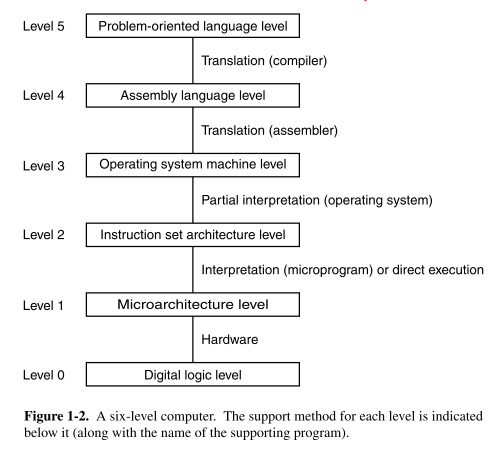
\includegraphics[scale=0.5]{levels-architecture-computer.png}

\begin{itemize}
	\item applicativo: linguaggi di alto livello utilizzati dai programmatori (es. C, C++, Python)
	\item sistema operativo: fornisce un'insieme di funzionalitá al livello applicativo (es. syscall, gestione della memoria)
	\item ISA (Instruction Set Architecture): insieme di istruzioni (instruction set) di uno specifico processore
	\item microarchitettura: interpretazione delle istruzioni ISA in microistruzioni (semplici istruzioni come fare la somma di due numeri)
	\item logico-digitale: hardware del calcolatore e le sue componenti elementari
\end{itemize}

\subsubsection{Traduzione dei programmi C, C++}
Generalmente, C e C++ vengono compilati (nulla vieta di utilizzare un interprete) e questo é generalmente il processo che porta da un file sorgente a un eseguibile:
\begin{enumerate}
	\item compilazione: i singoli file sorgenti sono compilati in file oggetto (estensione .obj o .o)
	\item linking: vengono risolti i riferimenti dei singoli file
\end{enumerate}
A questo punto é disponibile un eseguibile, che, se invocato, viene caricato in memoria, i riferimenti vengono trasformati in indirizzi di memoria e il programma viene eseguito.

\subsubsection{Macchine virtuali}
La \textit{virtualizzazione} é un meccanismo che permette di astrarre un determinato componente di un sistema. Oggi, é utilizzata in diversi modi:
\begin{itemize}
	\item hardware: vengono virtualizzate le componenti fisiche di un computer, riuscendo ad esempio ad ospitare sistemi operativi diversi contemporaneamente, emulandoli
	\item software: alcuni linguaggi, come Java, vengono compilati in un \textit{linguaggio macchina immaginario} (in questo caso chiamato bytecode). Il linguaggio intermedio viene interpretato da una macchina viruale (JVM=Java Virtual Machine), che traduce queste istruzioni nello specifiche istruzioni ISA. La macchina virtuale é un interprete, quindi generalmente piú lento di un compilatore, anche se utilizza tecniche di \textbf{compilazione just-in-time} (compila delle istruzioni a runtime, appena prima che vengano eseguite) e \textbf{caching} (non ritraduce codice giá tradotto)
\end{itemize}

\section{Rappresentazione digitale delle informazioni}

\subsection{Precisione finita}
I calcolatori moderni utilizzano segnali \textit{digitali} (lat. digitus, dito).\\
A causa dela limitazione della quantitá di memoria, il calcolatore utilizza numeri a \textit{precisione finita}, ovvero rappresentati con un numero finito di cifre. A causa di questo, é possibile, in operazioni aritmetiche, ottenere errori: \textbf{underflow} (il risultato dell'operazione é minore del piú piccolo valore rappresentabile), \textbf{overflow} (il risultato dell'operazione é maggiore del piú grande valore rappresentabile) e \textbf{non appartenenza} (il risultato non é nè troppo grande, nè troppo piccolo ma non appartiene all'insieme dei valori rappresentabili). Per questo, non sempre valgono la proprietá associativa ($a+(b+c)=(a+b)+c$) e distributiva ($a(b+c)=ab+ac$).

\subsection{Notazione posizionale base 2}
Per rappresentare i numeri, si utilizza la notazione posizionale in \textbf{base 2}: $\displaystyle \sum_{i=-k}^{n} d_i \cdot 2^i$ ($-k$ per indicare anche i numeri decimali).\\
Un \textit{byte} indica un insieme di 8 bit; sequenze piú lunghe di 1 byte sono dette \textit{word} (hanno lunghezza variabile). Il numero di configurazioni dato un numero $n$ di bit é $2^n$.

\subsection{Conversioni}
Le principali conversioni sono:
\begin{itemize}
	\item binario $\rightarrow$ decimale: si moltiplica la cifra $i$-esima per $2^i$ (es. $11010_2 = 1\cdot2^4 + 1\cdot2^3 + 1\cdot2^1 = 16+8+1 = 25_{10}$)
	\item binario $\rightarrow$ ottale: si raggruppano, a partire dalla virgola, i bit in gruppi di 3 e si convertono in una cifra del sistema ottale (perché $8=2^3$)
	\item binario $\rightarrow$ esadecimale: stessa cosa dell'ottale ma con gruppi di 4 cifre (perché $16=2^4$)
\end{itemize}

\subsection{Codifica dei numeri interi}
I numeri interi vengono rappresentati con due principali metodi:
\begin{itemize}
	\item complemento a 2
	\item eccesso $2^{m-1}$
\end{itemize}
Nel complemento a 2, dato un numero $n$, $-n$ é ottenibile invertendo ciascun bit di $n$ e aggiungendo 1. I numeri positivi hanno come primo bit 0, i negativi 1. Per ottenere il valore assoluto di un numero negativo, basta quindi applicare il complemento a 2.\\\\
Nella codifica eccesso $2^{m-1}$, un numero $n$ é rappresentato da $n + 2^{m-1}$, dove $m$ é il numero di bit utilizzati per rappresentare $n$. É identico al complemento a 2 con il bit di segno invertito: i numeri da $-2^{m-1}$ a $+2^{m-1}-1$ sono mappati da $0$ a $2^{m}-1$ (es. con 8 bit, i numeri da -127 a 128 sono mappati da 0 a 255).\\\\
Con entrambe queste codifiche si ha una sola rappresentazione per ciascun numero (compreso lo 0), oltre ai seguenti vantaggi:
\begin{itemize}
	\item possibilitá di utilizzare un \underline{unico circuito} sia per la somma che per la sottrazione, perchè $a-b=a+(-b)$
	\item per verificare se é avvenuto un overflow/underflow, é sufficiente controllare che gli ultimi 2 bit del riporto siano \underline{diversi}
\end{itemize}

\subsection{Mascheramento}
Una \textbf{maschera} é una qualsiasi configurazione di un insieme di bit di lunghezza predefinita. Il mascheramento consiste nell'utilizzo delle maschere e di operazioni bitwise per compiere determinate operazioni. Le operazioni piú comuni sono impostare dei bit a 1 (OR bitwise con una maschera che ha esclusivamente i bit da settare a 1) o 0 (AND bitwise con una maschera che ha esclusivamente i bit da settare a 0) e uverificare se dei bit sono impostati a 1 o 0 (AND bitwise con i bit da controllare a 1: se il rimanente é = 0, i bit erano impostati a 1, altrimenti a 0).

\subsection{Codifica dei numeri a virgola mobile}
Per rappresentare dei numeri con la virgola, si utilizza un sistema detto \textbf{floating-point} (virgola mobile):
$$n = f \times 10^e$$
dove f é detta \textit{mantissa} e determina la \underline{precisione}, $e$ é detto \textit{esponente} e determina la gamma dei \underline{valori rappresentabili}.\\
In questa notazione, esistono piú rappresentazioni per uno stesso numero, quindi si adotta la \textbf{codifica standard}, con $0.1 \le f < 1$.\\
Per quanto la gamma dei valori rappresentabili sia molto ampia, si hanno sempre un numero finito di cifre, quindi un numero finito di valori rappresentabili: quando il risultato non appartiene all'insieme dei numeri rappresentabili si commette un errore di arrotondamento $E = min(|v-v_1|;|v-v_2|)$ dove $v$ é il valore reale e $v_1, v_2$ i valori rappresentabili piú vicini ad esso.\\
L'errore assoluto aumenta all'aumentare del valore rappresentato, mentre l'errore relativo rimane costante.

\subsection{IEEE 754}
L'iEEE 754 é uno standard di codifica dei numeri in virgola mobile. I formati piú utilizzati sono:
\begin{itemize}
	\item \textbf{singola precisione}, 32 bit: 1 segno, 8 esponente, 23 mantissa
	\item \textbf{doppia precisione}, 64 bit: 1 segno, 11 esponente, 52 mantissa
\end{itemize}
L'esponente é rappresentato in eccesso $2^{m-1}-1$ (ad esempio in singola precisione é in eccesso $2^{8-1}-1=2^7-1=128-1=127$), siccome una configurazione é riservata a $+\infty,-\infty \mbox{ e } NaN$ (not a number)\footnote{esiste una distinzione ulteriore tra SNaN (signaling NaN) e QNaN (quiet nan): il primo, se utilizzato in operazioni aritmetiche, genera (se opportunamente configurato) un'eccezione}.\\\\
I numeri sono rappresentati in due forme:
\begin{itemize}
	\item forma \textbf{normalizzata}: nella mantissa binaria viene memorizzata solamente la parte decimale (\textit{fraction}); la mantissa viene implicitamente considerata 1,\textit{fraction}
	\item forma \textbf{denormalizzata}: utilizzata per rappresentare valori inferiori al minimo valore normalmente rappresentabile nella forma normalizzata, presenta tutti i bit dell'esponente a 0 e considera implicitamente la mantissa come 0,\textit{fraction}
\end{itemize}

\section{Architettura del calcolatore}
L'architettura di un calcolatore é il modo in cui sono organizzati e collegati i suoi componenti.

\subsection{Architettura di Von Neumann}
L'architettura piú utilizzata é la architettura di Von Neumann, basata sul fatto che anche le istruzioni dei \textbf{programmi}, oltre ai \textbf{dati}, sono salvati in memoria.\\
La CPU utilizza i \textbf{bus}, interconnessioni elettriche che permettono il trasferimento di informazioni, per gestirli. I due bus piú comuni sono il \textbf{bus dati} e il \textbf{bus indirizzi}. Esiste anche il \textbf{bus controlli} che serve per coordinare le attivitá del sistema e comunicare con i dispositivi inviando segnali.

\subsection{CPU}
La CPU si occupa di leggere le istruzioni dei programmi immagazzinati in memoria ed eseguirle. É composta da:
\begin{itemize}
	\item \textbf{unitá di controllo} (CU, control unit): legge le istruzioni in memoria centrale e ne identifica la tipologia
	\item \textbf{ALU} (arithmetic logic unit): esegue le operazioni aritmetico-logiche (es. somma, operazioni bitwise)
	\item \textbf{registri}: piccole aree di memoria ad alta velocitá utilizzate per memorizzare risultati temporanei di istruzioni e informazioni di controllo (es. flag)
\end{itemize}

\subsubsection{Registri}
Normalmente i registri hanno tutti la stessa dimensione. Inoltre, esistono dei registri general-purpose e altri che hanno uno scopo specifico, tra cui:
\begin{itemize}
	\item \textbf{program counter} (PC): contiene l'indirizzo della prossima istruzione da eseguire
	\item \textbf{instruction register} (IR): contiene l'indirizzo dell'istruzione corrente
\end{itemize}

\subsubsection{Ciclo di fetch-execute}
Per eseguire un'istruzione, la CPU compie il cosiddetto ciclo di \textbf{fetch-execute}:
\begin{enumerate}
	\item il valore del PC viene messo in \textbf{MAR} (memory address register) e ci si prepara alla lettura
	\item si accede all'indirizzo di memoria specificato in MAR e si scrive il valore letto su \textbf{MDR} (memory data register)
	\item il valore di MDR viene copiato in IR e l'istruzione viene decodificata
	\item l'istruzione viene passata all'ALU. In caso siano necessari degli operandi in ingresso, devono essere reperiti seguendo il processo di prima (indirizzo del primo operando su MAR, accesso in memoria e scrittura su MDR; stessa cosa per un eventuale secondo)
	\item il risultato dell'operazione viene salvato nel registro. In caso sia necessario salvare in memoria il risultato, si carica l'indirizzo di destinazione in MAR, si carica il risultato in MDR, si accede in memoria e si scrive il valore
	\item si aggiorna il program counter e si ricomincia
\end{enumerate}

\subsubsection{Ciclo di data path}
Con ciclo di \textbf{data path} si intende il passaggio di 2 operandi attraverso la ALU e la memorizzazione del risultato in un nuovo registro. Ogni istruzione assembly viene eseguita in uno o piú cicli di data path (es. divisione). In architetture non parallele, questo ciclo viene eseguito ogni ciclo di \textbf{clock}.

\end{document}